\section{التنفيذ}
\label{sec:implementation}

يتبع التنفيذ العملي ترتيب المراحل نفسه في مشغل سير العمل: تحميل البيانات، والبحث، وتوليد الاستطرادات، وتوليد النص الإخفائي، وفك الترميز. وتحتفظ كل مرحلة بمخرجاتها الوسيطة على القرص كي تتمكن المراحل اللاحقة من إعادة استخدام المدونة والتجزئات نفسها، مما يحافظ على اتساق المرسل والمستقبل عبر محاولات الإعادة.

\subsection{المكونات المعمارية}
يُشغَّل النظام عبر سلسلة من مراحل خطية حتمية. وتشمل المكونات الرئيسة:
\begin{itemize}
    \item \textbf{مرحلة تحميل البيانات:} تجلب محتوى الروابط غير المحلولة وتستبدل نص المنشور بالنص المستخرج.
    \item \textbf{مرحلة البحث:} تولد مصطلحات البحث من عنوان المنشور ونصه ورابطه باستخدام ضبط حتمي لنموذج اللغة، مثل \texttt{temperature=0}، ثم تستعلم واجهة بحث ذات صيغة ثابتة، وتحذف الروابط المكررة وملفات \EN{PDF}، وتجلب نصوص الصفحات في دفعات محدودة. وتحتفظ هذه المرحلة بمدونة مسطحة لنتائج البحث مع قيم تجزئة للتحقق من قابلية الإعادة.
    \item \textbf{مرحلة توليد الاستطرادات:} تسطح المدونة المجمعة من نص المنشور ومدونة نتائج البحث والتعليقات، ثم تستدعي مشغل الاستطرادات لإنتاج ثلاثيات تتألف من فئة، واقتباس مصدر، واستطرادة. وتقسم المدخلات الطويلة إلى مقاطع طولها 30 ألف محرف وترسل على دفعات حتى 150 ألف محرف. وإذا فشل مسار الواجهة الخلفية، يعود خط المعالجة إلى موجه مباشر لنموذج اللغة يستخدم مخطط \EN{JSON} نفسه.
    \item \textbf{مرحلتَا الإخفاء وفك الترميز:} تجمعان طبقة الضغط، واستهداف التعليق، والقائمة الدلالية المختصرة، وحلقة التحقق. يولد المرشح عددًا صغيرًا ثابتًا من التعليقات المرشحة للاستطرادة المختارة، ويفك ترميزها مباشرة، ويعيد التوليد إذا لم تكن الاستطرادة المختارة قابلة للاسترجاع.
\end{itemize}
يربط الشكل~\ref{fig:impl-pipelines} هذه المكونات بالمراحل المنفذة والمخرجات الوسيطة المخزنة على القرص.

\begin{figure*}[t]
	\centering
	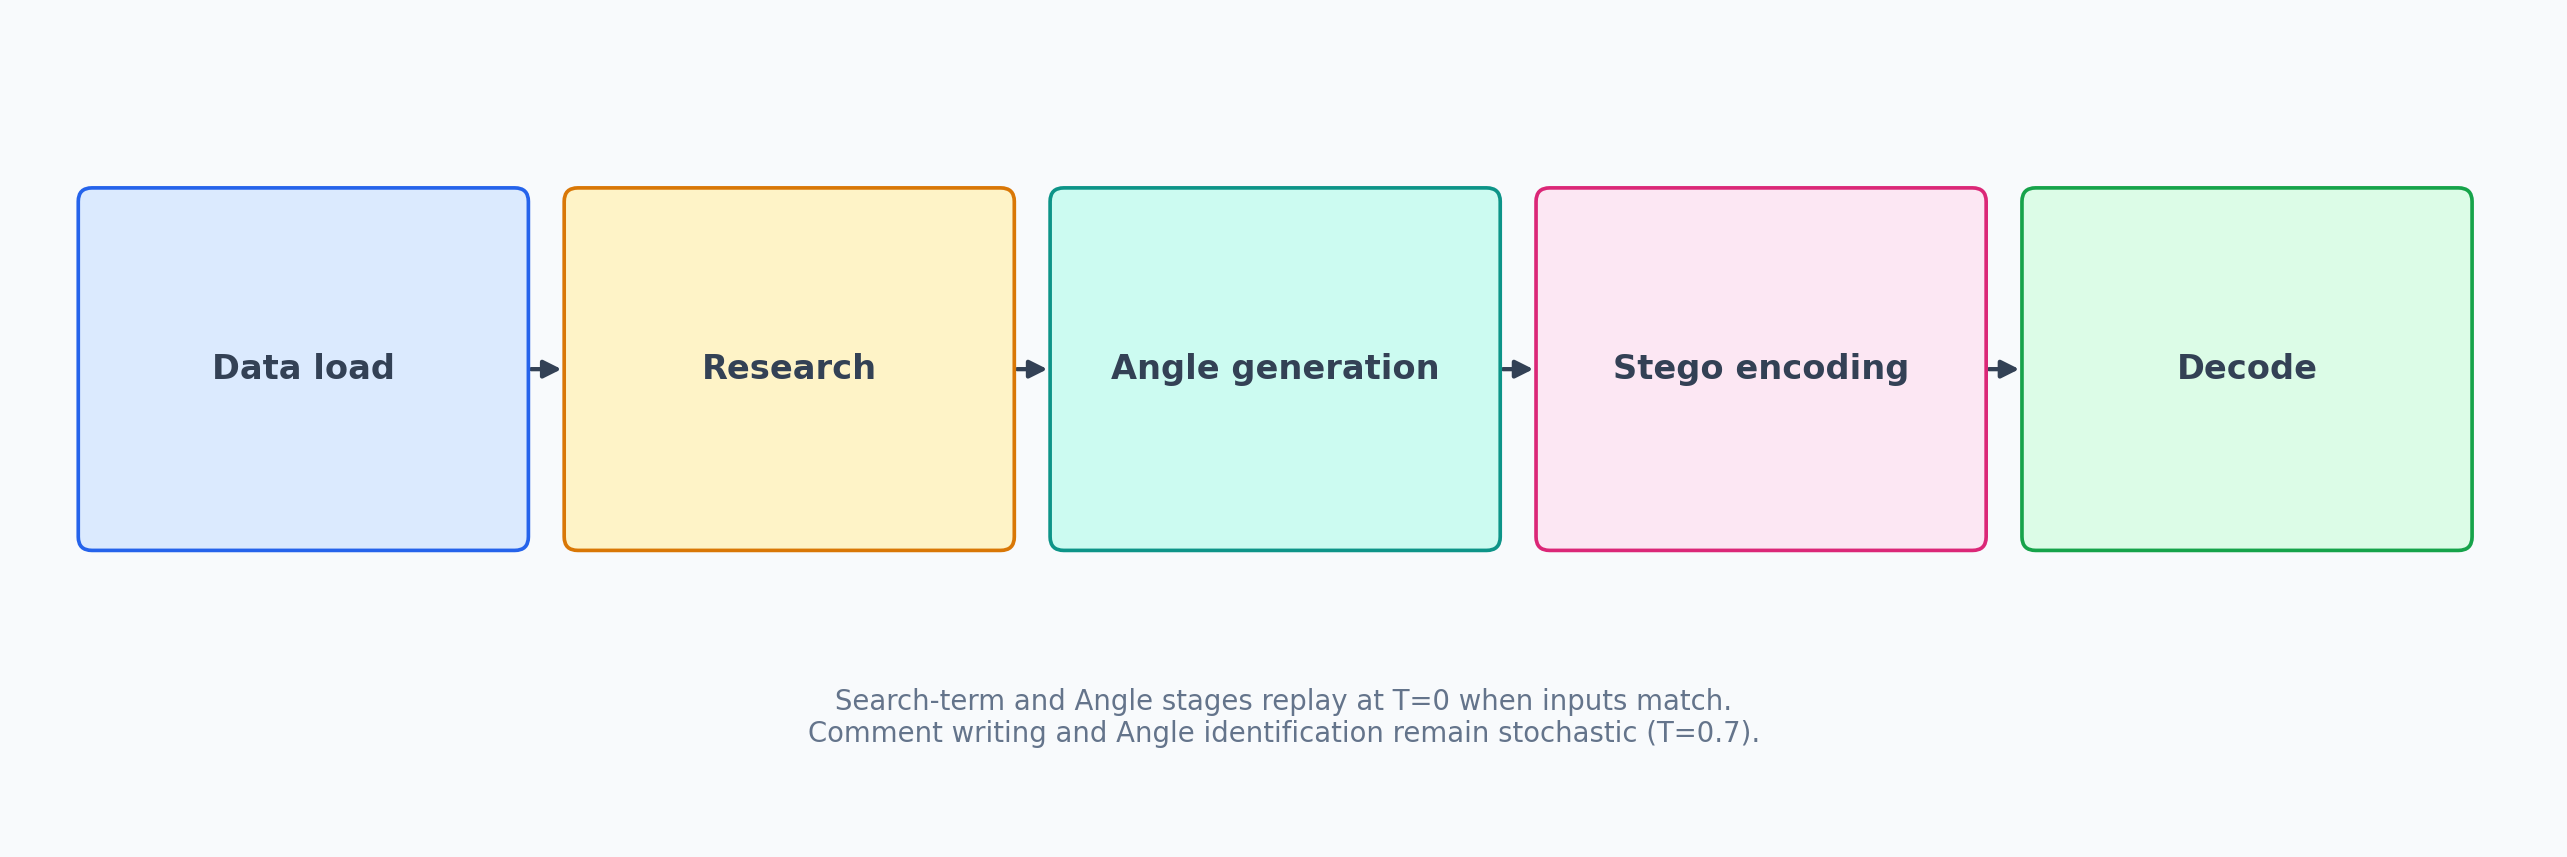
\includegraphics[width=\textwidth,height=0.55\textheight,keepaspectratio]{figures/implementation_pipelines}
	\caption{تتوافق مراحل التنفيذ والمخرجات المحفوظة مع المنهجية: كل مرحلة حتمية وقابلة للإعادة حيث يلزم ذلك للحفاظ على تماثل المرسل والمستقبل.}
	\label{fig:impl-pipelines}
\end{figure*}

\subsection{ضبط النماذج}
يستخدم التنفيذ أدوارا نموذجية مختلفة للمراحل المختلفة، لكن معرفات النماذج الدقيقة تعامل كمعاملات قابلة للضبط:
\begin{itemize}
    \item \textbf{المراحل الحتمية، مثل توليد المصطلحات والاستطرادات:} تعمل عند \texttt{temperature=0} لضمان إعادة بناء قابلة للتكرار من المدخلات نفسها.
    \item \textbf{توليد النص الإخفائي:} يعمل عند حرارة غير صفرية لتوليد ردود مرشحة متنوعة لاختيار تضمين ثابت.
    \item \textbf{المطابقة الدلالية وفك الترميز:} يستخدم نموذج تشابه دلالي لترتيب القائمة المختصرة، يتبعه موجه تحديد تمييزي حتمي، مثل \texttt{temperature=0}، لاختيار فهرس الاستطرادة النهائي.
\end{itemize}
